\documentclass{article}
\usepackage{tikz}
\usepackage{pgfplots}
\pgfplotsset{compat=1.18}
\usepackage{geometry}
\geometry{a4paper, margin=1cm} % Adjust margins to fit figures on one page if needed

\begin{document}

\begin{center}
\section*{Visualizing P2P ICP Solving Steps (TikZ Series)}
\end{center}

\vspace{1cm}

% --- FIGURE 1: Initial Point Clouds & Centroids ---
\begin{figure}[h]
\centering
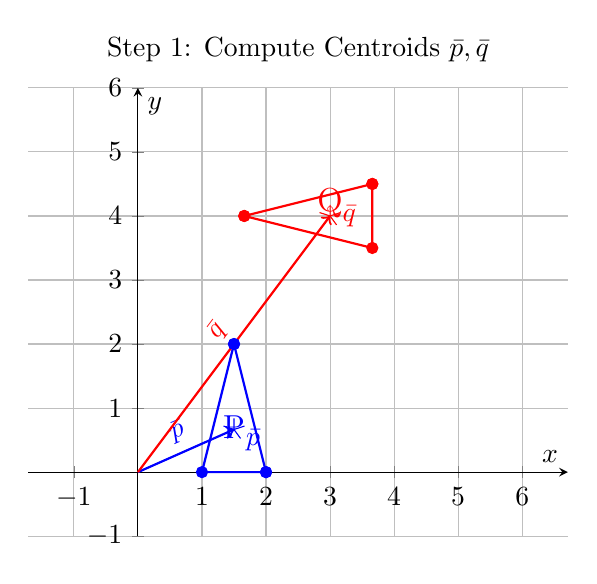
\begin{tikzpicture}
\begin{axis}[
    axis lines=middle,
    xmin=-1, xmax=6, ymin=-1, ymax=6,
    xtick={-1, 0, ..., 6}, ytick={-1, 0, ..., 6},
    axis equal, % Crucial for accurate shape comparison
    xlabel=$x$, ylabel=$y$,
    title={Step 1: Compute Centroids \(\bar{p}, \bar{q}\)},
    grid=both
]
% Point Cloud P (Source) - Offset Blue Triangle
\addplot[mark=*, blue, only marks, mark size=2pt] coordinates {(1,0) (2,0) (1.5, 2)} node[anchor=north] at (1,0) {}; % P1
\addplot[mark=*, blue, only marks, mark size=2pt] coordinates {(2,0)} node[anchor=north] at (2,0) {}; % P2
\addplot[mark=*, blue, only marks, mark size=2pt] coordinates {(1.5,2)} node[anchor=south] at (1.5,2) {}; % P3
\draw[blue, thick] (axis cs:1,0) -- (axis cs:2,0) -- (axis cs:1.5,2) -- cycle;
\node[blue, font=\large] at (axis cs:1.5,0.7) {P};

% Centroid p_bar (mark with star)
\addplot[mark=star, blue, mark size=4pt] coordinates {(1.5, 0.666)}; % Calculated p_bar (approx)
\draw[blue, ->, thick] (axis cs:0,0) -- (axis cs:1.5, 0.666) node[midway, sloped, above] {\(\bar{p}\)};
\node[blue] at (axis cs:1.8, 0.5) {\(\bar{p}\)};

% Point Cloud Q (Target) - Offset/Rotated Red Triangle (90deg CCW, translate to (3,4))
\addplot[mark=*, red, only marks, mark size=2pt] coordinates {(3.66,3.5) (3.66,4.5) (1.66,4)} node[anchor=south] at (3.66,3.5) {}; % Q1 (rotated/translated P1 relative to its centroid?) - Wait, let's make it simple. Let Q be P rotated 90deg CCW and shifted.
\addplot[mark=*, red, only marks, mark size=2pt] coordinates {(3.66,4.5)} node[anchor=west] at (3.66,4.5) {}; % Q2
\addplot[mark=*, red, only marks, mark size=2pt] coordinates {(1.66,4)} node[anchor=south] at (1.66,4) {}; % Q3
\draw[red, thick] (axis cs:3.66,3.5) -- (axis cs:3.66,4.5) -- (axis cs:1.66,4) -- cycle;
\node[red, font=\large] at (axis cs:3,4.2) {Q};

% Centroid q_bar (mark with star, translate centroid to (3,4))
\addplot[mark=star, red, mark size=4pt] coordinates {(3, 4)}; % target q_bar
\draw[red, ->, thick] (axis cs:0,0) -- (axis cs:3, 4) node[midway, sloped, above] {\(\bar{q}\)};
\node[red] at (axis cs:3.3, 4) {\(\bar{q}\)};

\end{axis}
\end{tikzpicture}
\caption{Initial Point Clouds P (blue, offset triangle) and Q (red, offset and rotated triangle), with their calculated centroids \(\bar{p}\) and \(\bar{q}\) marked and vectors from the origin shown.}
\label{fig:initial}
\end{figure}

\vspace{1cm}

% --- FIGURE 2: Centering (Conceptual) for H ---
\begin{figure}[h]
\centering
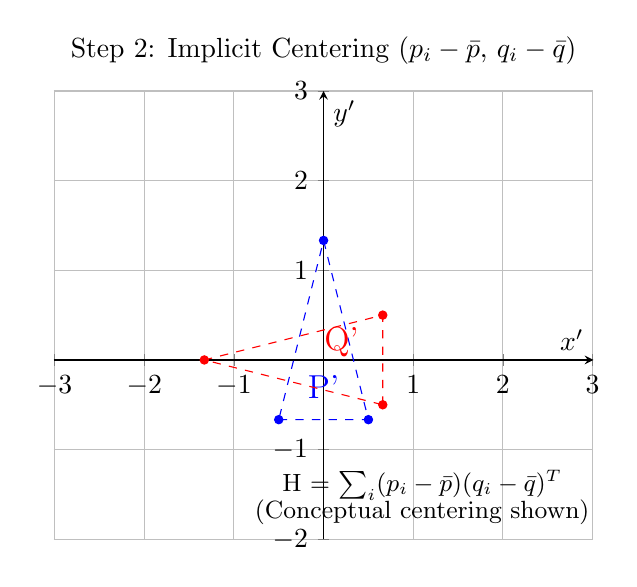
\begin{tikzpicture}
\begin{axis}[
    axis lines=middle,
    xmin=-3, xmax=3, ymin=-2, ymax=3,
    xtick={-3, -2, ..., 3}, ytick={-2, -1, ..., 3},
    axis equal,
    xlabel=$x'$, ylabel=$y'$,
    title={Step 2: Implicit Centering (\(p_i - \bar{p}\), \(q_i - \bar{q}\))},
    grid=both
]
% Point Cloud P' (Centered at Origin)
\addplot[mark=*, blue, only marks, mark size=1.5pt] coordinates {(-0.5,-0.666) (0.5,-0.666) (0, 1.333)}; % P'_i
\draw[blue, thin, dashed] (axis cs:-0.5,-0.666) -- (axis cs:0.5,-0.666) -- (axis cs:0, 1.333) -- cycle;
\node[blue, font=\large] at (axis cs:0, -0.3) {P'};

% Point Cloud Q' (Centered at Origin, retains relative rotation)
\addplot[mark=*, red, only marks, mark size=1.5pt] coordinates {(0.66, -0.5) (0.66, 0.5) (-1.33, 0)}; % Q'_i (rotated centered P')
\draw[red, thin, dashed] (axis cs:0.66, -0.5) -- (axis cs:0.66, 0.5) -- (axis cs:-1.33, 0) -- cycle;
\node[red, font=\large] at (axis cs:0.2, 0.2) {Q'};

\node[font=\small] at (axis cs: 1.1, -1.4) {H = \(\sum_i (p_i-\bar{p})(q_i-\bar{q})^T\)};
\node[font=\small] at (axis cs: 1.1, -1.7) {(Conceptual centering shown)};

\end{axis}
\end{tikzpicture}
\caption{Visualization of Step 2 conceptually centering both point clouds at the global origin to compute the cross-covariance matrix H using the relative positions of points to their respective centroids.}
\label{fig:centering}
\end{figure}

\vspace{1cm}

% --- FIGURE 3: SVD Components (Principle Axes) ---
\begin{figure}[h]
\centering
\begin{minipage}{0.48\textwidth}
\centering
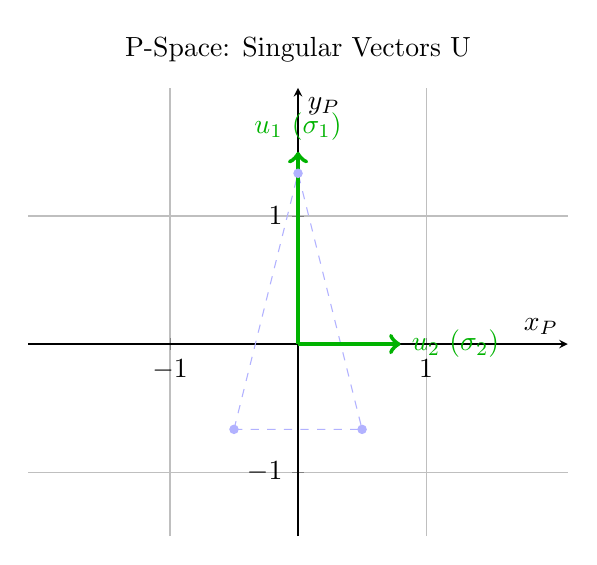
\begin{tikzpicture}
\begin{axis}[
    axis lines=middle,
    xmin=-1.5, xmax=1.5, ymin=-1.5, ymax=2,
    xtick={-1, 0, 1}, ytick={-1, 0, 1},
    axis equal,
    xlabel=$x_P$, ylabel=$y_P$,
    title={P-Space: Singular Vectors U},
    grid=both
]
% Centered P' points for context (faint)
\addplot[mark=*, blue!30!white, only marks, mark size=1.5pt] coordinates {(-0.5,-0.666) (0.5,-0.666) (0, 1.333)};
\draw[blue!30!white, thin, dashed] (axis cs:-0.5,-0.666) -- (axis cs:0.5,-0.666) -- (axis cs:0, 1.333) -- cycle;

% Orthogonal Singular Vectors U (illustrative, not precise for these specific points)
\draw[green!70!black, ->, ultra thick] (axis cs:0,0) -- (axis cs:0, 1.5) node[anchor=south] {\(u_1\) (\(\sigma_1\))};
\draw[green!70!black, ->, ultra thick] (axis cs:0,0) -- (axis cs:0.8, 0) node[anchor=west] {\(u_2\) (\(\sigma_2\))};

\end{axis}
\end{tikzpicture}
\end{minipage}
\hfill
\begin{minipage}{0.48\textwidth}
\centering
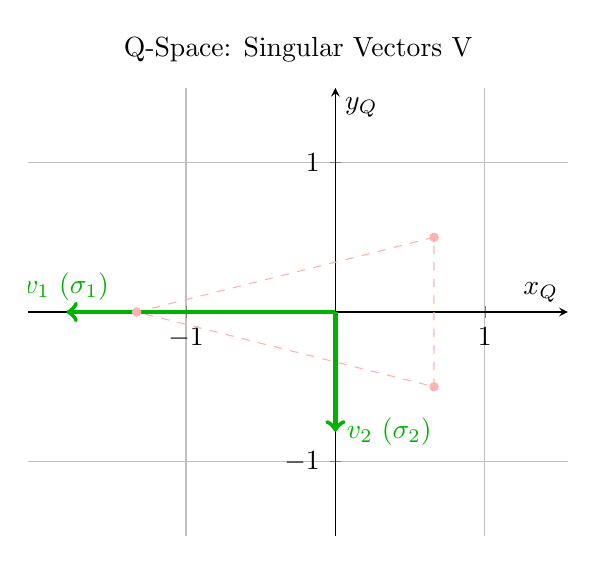
\begin{tikzpicture}
\begin{axis}[
    axis lines=middle,
    xmin=-2, xmax=1.5, ymin=-1.5, ymax=1.5,
    xtick={-1, 0, 1}, ytick={-1, 0, 1},
    axis equal,
    xlabel=$x_Q$, ylabel=$y_Q$,
    title={Q-Space: Singular Vectors V},
    grid=both
]
% Centered Q' points for context (faint)
\addplot[mark=*, red!30!white, only marks, mark size=1.5pt] coordinates {(0.66, -0.5) (0.66, 0.5) (-1.33, 0)};
\draw[red!30!white, thin, dashed] (axis cs:0.66, -0.5) -- (axis cs:0.66, 0.5) -- (axis cs:-1.33, 0) -- cycle;

% Orthogonal Singular Vectors V (illustrative, aligned relative to Q' similarly to U for P', but rotated)
\draw[green!70!black, ->, ultra thick] (axis cs:0,0) -- (axis cs:-1.8, 0) node[anchor=south] {\(v_1\) (\(\sigma_1\))};
\draw[green!70!black, ->, ultra thick] (axis cs:0,0) -- (axis cs:0, -0.8) node[anchor=west] {\(v_2\) (\(\sigma_2\))};

\end{axis}
\end{tikzpicture}
\end{minipage}
\caption{Visualization of Step 3 SVD decomposition \(H = U\Sigma V^T\), showing the orthogonal singular vectors U and V as principal axes in the centered frames of reference for P and Q respectively, with illustrative singular values \(\sigma_i\) indicating the scale of variance along these directions.}
\label{fig:svd}
\end{figure}

\vspace{1cm}

% --- FIGURE 4: Rotation R (on centered shape) ---
\begin{figure}[h]
\centering
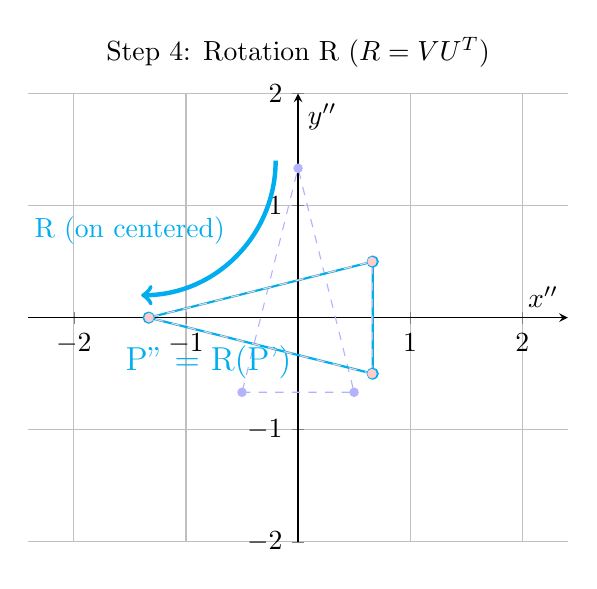
\begin{tikzpicture}
\begin{axis}[
    axis lines=middle,
    xmin=-2, xmax=2, ymin=-2, ymax=2,
    xtick={-2, -1, ..., 2}, ytick={-2, -1, ..., 2},
    axis equal,
    xlabel=$x''$, ylabel=$y''$,
    title={Step 4: Rotation R (\(R = VU^T\))},
    grid=both
]
% Start with Centered P' (faint dashed)
\addplot[mark=*, blue!30!white, only marks, mark size=1.5pt] coordinates {(-0.5,-0.666) (0.5,-0.666) (0, 1.333)};
\draw[blue!30!white, thin, dashed] (axis cs:-0.5,-0.666) -- (axis cs:0.5,-0.666) -- (axis cs:0, 1.333) -- cycle;

% Show Rotation Action (Conceptually align U with V from previous step)
\draw[->, cyan, ultra thick, bend left=45] (axis cs: -0.2, 1.4) to node[midway, above left, cyan] {R (on centered)} (axis cs: -1.4, 0.2);

% Rotated Centered P'' = R(P') (show new position/orientation in different color, e.g., cyan)
% Apply 90deg CCW rotation to centered P': (-0.5,-0.666)->(0.666,-0.5), (0.5,-0.666)->(0.666,0.5), (0,1.333)->(-1.333,0)
\addplot[mark=*, cyan, only marks, mark size=2pt] coordinates {(0.666,-0.5) (0.666,0.5) (-1.333,0)};
\draw[cyan, thick] (axis cs:0.666,-0.5) -- (axis cs:0.666,0.5) -- (axis cs:-1.333,0) -- cycle;
\node[cyan, font=\large] at (axis cs: -0.8, -0.4) {P'' = R(P')};

% Target Centered Q' (faint red dashed, shows perfect shape alignment)
\addplot[mark=*, red!20!white, only marks, mark size=1.5pt] coordinates {(0.66, -0.5) (0.66, 0.5) (-1.33, 0)};
\draw[red!20!white, thin, dashed] (axis cs:0.66, -0.5) -- (axis cs:0.66, 0.5) -- (axis cs:-1.33, 0) -- cycle;

\end{axis}
\end{tikzpicture}
\caption{Visualizing Step 4 rotation part, showing how the rotation matrix R is conceptually applied to the centered point cloud P' to align its principal axes with those of centered Q', resulting in the rotated, centered shape P''.}
\label{fig:rotation}
\end{figure}

\vspace{1cm}

% --- FIGURE 5: Translation t & Final Alignment ---
\begin{figure}[h]
\centering
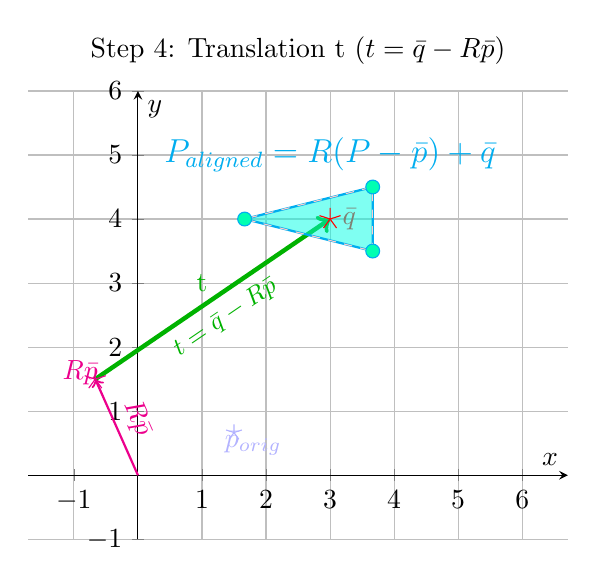
\begin{tikzpicture}
\begin{axis}[
    axis lines=middle,
    xmin=-1, xmax=6, ymin=-1, ymax=6,
    xtick={-1, 0, ..., 6}, ytick={-1, 0, ..., 6},
    axis equal,
    xlabel=$x$, ylabel=$y$,
    title={Step 4: Translation t (\(t = \bar{q} - R\bar{p}\))},
    grid=both
]
% Original p_bar (mark with faint star)
\addplot[mark=star, blue!30!white, mark size=3pt] coordinates {(1.5, 0.666)};
\node[blue!30!white] at (axis cs:1.8, 0.5) {\(\bar{p}_{orig}\)};

% Conceptually apply global rotation to p_bar to get R(p_bar)
% Since p_bar -> 0 (centering), R(0) = 0. So the global rotation R applies *around origin*.
% For p_bar=(1.5, 0.666), apply 90deg CCW rotation about origin (assume this is R): R(p_bar) = (-0.666, 1.5)
\addplot[mark=star, magenta, mark size=4pt] coordinates {(-0.666, 1.5)}; % R(p_bar)
\draw[magenta, ->, thick] (axis cs:0,0) -- (axis cs:-0.666, 1.5) node[midway, sloped, above] {\(R\bar{p}\)};
\node[magenta] at (axis cs:-0.9, 1.6) {\(R\bar{p}\)};

% Target q_bar
\addplot[mark=star, red, mark size=4pt] coordinates {(3, 4)};
\node[red] at (axis cs:3.3, 4) {\(\bar{q}\)};

% Translation vector t = q_bar - R(p_bar) (draw vector from R(p_bar) to q_bar)
\draw[green!70!black, ->, ultra thick] (axis cs:-0.666, 1.5) -- (axis cs:3, 4) node[midway, sloped, below, font=\small] {\(t = \bar{q} - R\bar{p}\)};
\node[green!70!black] at (axis cs: 1, 3) {t};

% --- Conceptual Final Perfect Alignment (Show result) ---
% Shift rotated, centered shape P'' (Fig 4, cyan) by q_bar to q_bar position.
\addplot[mark=*, cyan, only marks, mark size=2.5pt, fill=green!30!cyan] coordinates {(3.666,3.5) (3.666,4.5) (1.666,4)};
\draw[cyan, thick, fill=green!10!cyan, fill opacity=0.5] (axis cs:3.666,3.5) -- (axis cs:3.666,4.5) -- (axis cs:1.666,4) -- cycle;
\node[cyan, font=\large] at (axis cs: 3, 5) {\(P_{aligned} = R(P-\bar{p}) + \bar{q}\)};

% original Q for comparison (faint dashed red)
\draw[red!20!white, thin, dashed] (axis cs:3.66,3.5) -- (axis cs:3.66,4.5) -- (axis cs:1.66,4) -- cycle;

\end{axis}
\end{tikzpicture}
\caption{Visualizing the Step 4 translation vector calculation t = \(\bar{q} - R\bar{p}\). The vector t shifts the rotated source centroid \(R\bar{p}\) directly to the target centroid \(\bar{q}\). Conceptual perfect shape alignment (cyan filled triangle) is shown centered on \(\bar{q}\), aligning with the original Q shape.}
\label{fig:translation}
\end{figure}

\end{document}